\subsection{Translation and Ribosomal Synthesis}
Lastly, we turn our attention to the process of synthesizing new proteins,
translation. This process stands as a good candidate for potentially limiting growth
since the synthesis of new proteins relies on the generation of ribosomes,
themselves proteinaceous molecules. As we will see in the coming sections of
this work, this poses a "chicken-or-the-egg" problem where the synthesis of
ribosomes requires ribosomes in the first place.

We will begin our exploration of protein translation in the same spirit as we
have in previous sections -- we will draw order-of-magnitude estimates based on
our intuition and available literature, and then compare these estimates
to the observed data. In doing so, we will estimate both the absolute number of
ribosomes necessary for replication of the proteome as well as the synthesis of
amino-acyl tRNAs. From there we consider the limitations on ribosomal synthesis in
light of our estimates on both the synthesis of ribosomal proteins and
our earlier results on rRNA synthesis.

\subsubsection{tRNA Synthetases}
We begin by first estimating the number of tRNA synthetases in \textit{E. coli}
needed to convert free amino-acids to polypeptide chains. At a modest growth
rate of $\approx$ 5000 s, \textit{E. coli} has roughly 3$\times$10$^6$ proteins
per cell (BNID: 115702; \cite{milo2010}). Assuming that the typical protein is
on the order of $\approx$ 300 amino acids in length (BNID: 100017;
\cite{milo2010}), we can estimate that a total of $\approx$ 10$^9$ amino acids
are stitched together by peptide bonds.

How many tRNAs are needed to facilitate this remarkable number of amino acid
delivery events to the translating ribosomes? It is important to note that tRNAs
are recycled after they've passed through the ribosome and can be recharged with
a new amino acid, ready for another round of peptide bond formation. While some
\textit{in vitro} data exists on  the turnover of tRNA in \textit{E. coli} for
different  animo acids, we can make a reasonable estimate by comparing the
number of amino acids to be  polymerized to cell division time. Using our
stopwatch of 5000 s and 10$^9$ amino acids, we arrive at a requirement of
$\approx$ 2 $\times$ 10$^5$ tRNA molecules. This estimate is in line with
experimental measurements of $\approx$ 3 $\times$ 10$^5$ per cell (BNID: 108611,
\cite{milo2010}), suggesting we are on the right track.

There  are many processes which go into synthesizing a tRNA and ligating it
with the appropriate amino acids. As we covered  in the previous section, there
appear to be more than enough RNA polymerases per cell to synthesize the needed
pool of tRNAs. Without considering the many ways in which amino acids can be
scavenged or synthesized \textit{de novo}, we can explore ligation the as a potential rate limiting
step. The enzymes which link the correct amino acid to the tRNA, known as tRNA
synthetases or tRNA ligases, are incredible in their proofreading of substrates
with the incorrect amino acid being ligated once out of every $10^4$ to $10^5$
times (BNID: 103469, \cite{milo2010}). This is due in part to the consumption of
energy  as well as a multi-step pathway to ligation. While the rate at which
tRNA is ligated is highly dependent on the identity of the amino acid, it is
reasonable to state that the typical tRNA synthetase has charging rate of
$\approx$ 20 AA per tRNA synthetase per second (BNID: 105279, \cite{milo2010}).

Combining these estimates together, as shown schematically in
\FIG{protein_synthesis}(A), yields an estimate of $\approx$ 10$^4$ tRNA
synthetases per cell with a division time of 5000 s. This point estimate is in
very close agreement with the observed number of synthetases (the sum of all 20
tRNA synthetases in \textit{E. coli}). This estimation strategy seems to
adequately describe the observed growth rate dependence of the tRNA synthetase copy
number (shown as the grey line in \FIG{protein_synthesis}(B)), suggesting that
the copy number scales with the cell volume.

In total, the estimated and observed $\approx$ 10$^4$ tRNA synthetases occupy
only a meager fraction of the total cell proteome, around 0.5\% by abundance. It
is reasonable to assume that if tRNA charging was a rate limiting process, cells
would be able to increase their growth rate by devoting more cellular resources
to making more tRNA synthases. As the synthesis of tRNAs and the corresponding
charging can be highly parallelized, we can argue that tRNA charging is not a
rate limiting step in cell division, at least for the growth conditions explored
in this work.

\subsubsection{Protein Synthesis}
With the number of tRNA synthetases accounted for, we now consider the abundance
of the protein synthesis machines themselves, ribosomes. Ribosomes are enormous
protein/rRNA complexes that facilitate the peptide bond formation between amino
acids in the correct sequence as defined by the coding mRNA. Before we examine
the synthesis of the ribosome proteins and the limits that may place on the
observed bacterial growth rates, let's consider replication of the cellular
proteome.

As described in the previous section, an \textit{E. coli} cell consisting of
of $\approx$ 3$\times$10$^6$ proteins will have on the order $\approx 10^9$
peptide bonds per proteome. While the rate at which ribosomes translates is
well known to have a growth rate dependence \cite{dai2018} and is a topic
which we discuss in detail in the coming sections. However, for the purposes
of our order-of-magnitude estimate, we can make the approximation that
translation occurs at a rate of $\approx$ 15 amino acids per second per
ribosome (BNID: 100233, \cite{milo2010}). Under this approximation and
assuming a division time of 5000 s, we can arrive at an estimate of
$\approx 10^4$ ribosomes are needed to replicate the cellular proteome,
shown in \FIG{protein_synthesis}(B). This point estimate, while glossing over
important details such as chromosome copy number and growth-rate dependent
translation rates, proves to be notably accurate when compared to the
experimental observations (\FIG{protein_synthesis}(B)).

\begin{figure}
    \begin{fullwidth}
    \centering{
        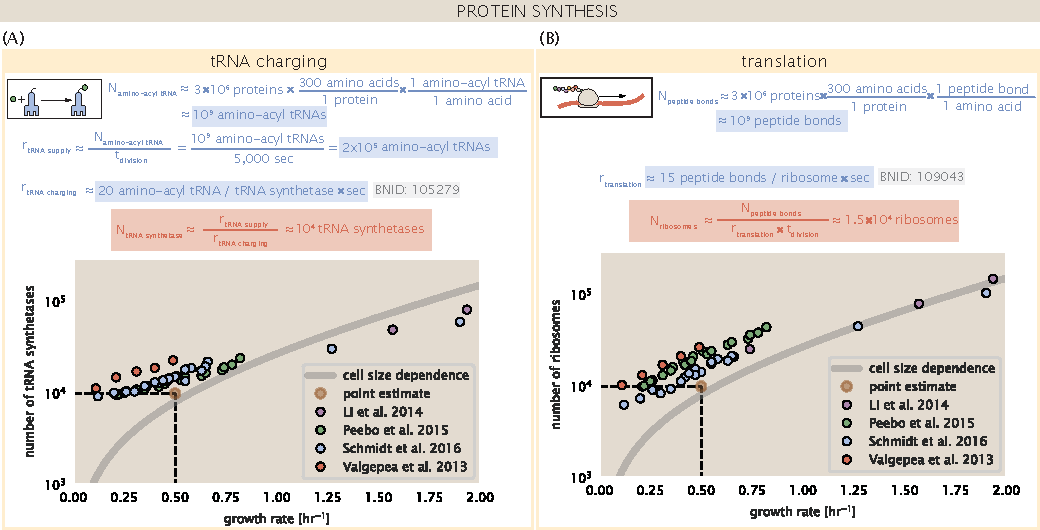
\includegraphics{main_figs/fig8_protein_synthesis.pdf}
        \caption{\textbf{Estimation of the required tRNA synthetases and
        ribosomes.} (A) Estimation for the
        number of tRNA synthetases that will supply the required amino acid
        demand. The sum of all tRNA synthetases copy numbers are plotted as a
        function of growth rate ([ArgS], [CysS], [GlnS], [GltX], [IleS], [LeuS],
        [ValS], [AlaS]$_2$, [AsnS]$_2$, [AspS]$_2$, [TyrS]$_2$, [TrpS]$_2$,
        [ThrS]$_2$, [SerS]$_2$, [ProS]$_2$, [PheS]$_2$[PheT]$_2$, [MetG]$_2$,
        [lysS]$_2$, [HisS]$_2$, [GlyS]$_2$[GlyQ]$_2$). (B) Estimation of the
        number of ribosomes required to synthesize 10$^9$ peptide bonds with an
        elongation rate of 15 peptide bonds per second. The
        average abundance of ribosomes is plotted as a function of growth rate.
        Our estimated values are shown for a growth rate of 0.5 hr$^{-1}$.
        Grey lines correpsond to the estimated complex abundance calculated at
        different growth rates. See Supplemental Information XX for a more
        detail description of this calculation.}
    \label{fig:protein_synthesis}
    }
    \end{fullwidth}
\end{figure}

\subsubsection{Translation as a Growth-Rate Limiting Step}
Thus far, the general back-of-the-envelope estimates have been
reasonably successful in explaining what sets the scale of absolute protein copy
number. A recurring theme that has arisen is the ability of cells to parallelize
their biosynthesis tasks. For example, while DNA replication speed-limit is
$\approx$ 40 minutes to replicate a genome, cells can divide faster than this by
initiating more than one round of replication per doubling. However, as we will
see, parallelization is not possible when it comes to the translation of
ribosomal proteins (\FIG{ribosome_limit}(A)). Thus, it is plausible that  translation may be a key factor in
determining the cellular growth rate.

% In many cases, these estimates can be adapted to consider a continuum of
% growth rates in lieu of our single 5000 s point estimate, the details of which are
% described in the Supplemental Information.
% growth on different carbon sources
% is achieved by inducing the expression of
% resulted in the induced
% expression of particular transporters, often producing more
% than needed to acquire enough carbon to build new cell mass (\FIG{carbon_transport}(B)). In
% examining replication of the DNA, we described how cells can replicate multiple
% copies of the chromosome at any given time, permitting growth rates faster than
% the limit at which the chromosome can be faithfully replicated.
% As another related example, we showed how increasing the gene dosage of the rRNA operons is
% necessary to produce enough rRNA to form functional ribosomes.

%
% Understanding the allocation of resources and large-scale structure of bacterial
% proteome has been an area of intense quantitative study over the last decade by Hwa and others
% \citep{scott2010, hui2015}. From the perspective of limiting growth, our
% earlier estimate of rRNA highlighted the necessity for multiple copies of
% rRNA genes in order to make enough rRNA. For \textit{E. coli}'s fastest
% growth rates at 2 hr$^{-1}$, the additional demand for rRNA is further
% supported by parallelized DNA replication and increased rRNA gene dosage.
% This suggests the possibility that synthesis of ribosomes might become rate
% limiting.

To gain some intuition into how translation can set the speed of
bacterial growth, we again consider the total number of peptide bonds that must
be synthesized, which we denote as $N_\text{AA}$. Noting that cells grow exponentially in time
\citep{godin2010}, we can compute the number of amino acids to be polymerized as
\begin{equation}
    N_\text{AA} \lambda = r_t R,
\end{equation} where
$\lambda$ is the cell growth rate in s$^{-1}$, $r_t$ is the maximum translation
rate in AA$\cdot$s$^{-1}$, and $R$ is the average ribosome copy number per
cell. Knowing the number of peptide bonds to be formed permits us to compute the
translation-limited growth rate as
\begin{equation}
\lambda_\text{translation-limited} = \frac{r_t R}{N_\text{AA}}.
\end{equation}

Alternatively, since $N_{AA}$ is related to the total protein mass through the
molecular weight of each protein, we can also consider the growth rate in terms
of the fraction of the total proteome mass that is dedicated to ribosomal
protein mass. By making the approximation that an average amino acid has a
molecular weight of 110 Da (BNID: 104877, \cite{milo2010}), we can approximate  $R
/ N_\text{AA} \approx \Phi_R / L_R$,  where $\Phi_R$ is the ribosomal mass
fraction and $L_R$ is the total length in amino acids that make up a ribosome.
The translation-limited growth rate can then be written in the form
\begin{equation}
\lambda_{\textrm{translation-limited}} \approx \frac{r_t}{L_R}  \Phi_R.
\label{eq:translation_limit_growth_rate}
\end{equation}
This is plotted as a function of ribosomal fraction $\Phi_R$ in
\FIG{ribosome_limit}(B), where we take $L_R \approx$ 7500 AA, corresponding to
the length in amino acids for all ribosomal subunits of the 50S and 30S complex
(BNID: 101175, \citep{milo2010}).

The growth rate defined by \EQ{translation_limit_growth_rate}
reflects mass-balance under steady-state growth and has long provided a
rationalization of the apparent linear increase in \textit{E. coli}'s ribosomal
content as a function of growth rate \citep{Goldberger1979, scott2010}.
We note that there is a maximum growth rate of $\lambda \approx 8
\,\text{hr}^{-1}$, or a doubling time just under 6 minutes
(\FIG{ribosome_limit}(B), dashed line). This represents an inherent speed limit
due to the need for the cell to double its entire ribosomal mass. Interestingly,
this limit is independent of the absolute number of ribosomes and is simply
given by the time to translate an entire ribosome, $L_R/ r_t$. As shown in
\FIG{ribosome_limit}(A), we can reconcile this with the observation that in
order to double the average number of ribosomes, each ribosome must produce a
second ribosome and cannot be parallelized.

\begin{figure}
  \begin{fullwidth}
        \centering{
            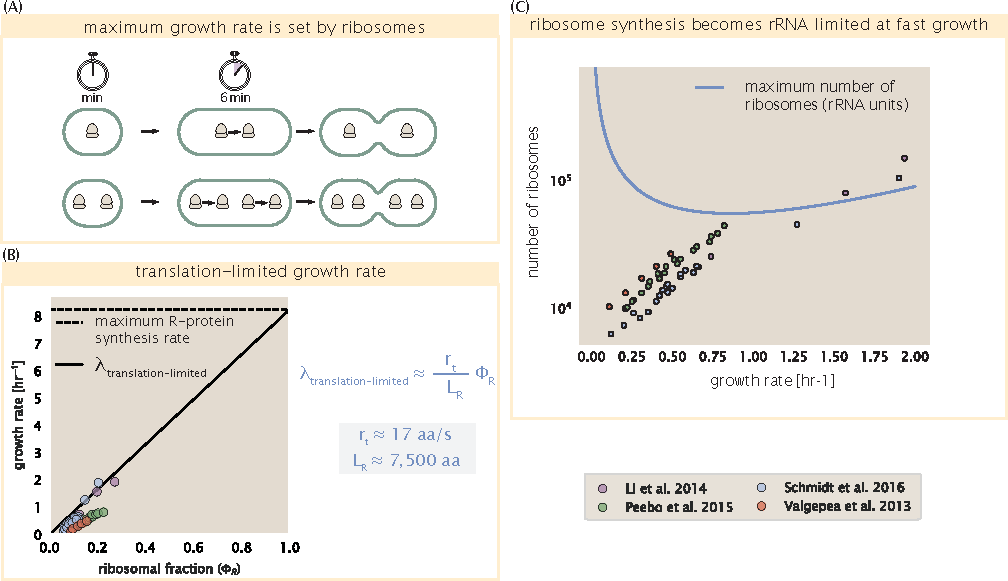
\includegraphics{main_figs/fig7_ribosome_growth_limit_2.pdf}
            \caption{\textbf{Translation-limited growth rate.} (A) Here we
            consider the translation-limited growth as a function of ribosomal
            fraction. By mass balance, the time required to double the entire
            proteome ($N_{AA}$ /$r_t$) sets the translation-limited
            growth rate, $\lambda_{\textrm{translation-limited}}$. Here $N_{aa}$
            is effectively the number of peptide bonds that must be translated,
            $r_t$ is the translation elongation rate, and $R$ is the number of
            ribosomes. This can also be re-written in terms of the ribosomal
            mass fraction $\Phi_R = m_R$ / $m_{\textrm{protein}}$, where $m_R$
            is the total ribosomal mass and $m_{\textrm{protein}}$ is the mass
            of all proteins in the cell. $L_R$ refers to the summed length of
            the ribosome in amino acids.
            $\lambda_{\textrm{translation-limited}}$ is plotted as a function of
            $\Phi_R$ (solid line). (B) The dashed line in part (A) identifies a
            maximum growth rate that is set by the ribosome. Specifically, this
            growth rate corresponds to the time required to  translation an
            entire ribosome, $L_R/ r_t$ . This is a result that is independent
            of the number of ribosomes in the cell as shown schematically here.
            (C) Maximum number of rRNA units that can be synthesized as
            as a function of growth rate. Solid curve corresponds to the rRNA
            copy number is calculated by multipyling the number of rRNA
            operons by the estimated number of $\langle\text{\# ori}\rangle$
            at each growth rate. The quantity $\langle\text{\# ori}\rangle$ was calculated
            using Equation 4 and the measurements from \cite{si2017} that are
            plotted in \FIG{translation_ecoli_partA}(A). Dashed line show that maximal number of
            functional rRNA units produced
            from a single chromosome without parallelization.            }
        \label{fig:ribosome_limit}
        }
  \end{fullwidth}
\end{figure}

% For reasonable values of $\Phi_R$, between about 0.1 - 0.3 \citep{scott2010},
% the maximum growth rate is in line with experimentally reported growth rates
% around 0.5 - 2 hr$^{-1}$. Importantly, in order for a cell to increase their
% growth limit they \textit{must} increase their relative ribosomal abundance.
% This can be achieved by either synthesizing more ribosomes or reducing the
% fraction of non-ribosomal proteins. Reduction of non-ribosomal proteins is not a
% straightforward task since (as we have found throughout our estimates) doubling
% a cell requires many other enzymes and transporters. Increasing the absolute
% ribosomal abundance in \textit{E. coli} will be limited by the number of rRNA
% operons.

Earlier, we considered rRNA synthesis (see Section \textit{\bf RNA
Synthesis}), finding that, when the rRNA operons are maximally loaded with
RNA polymerase, the cell can produce $\approx$ 1 functional rRNA unit per
second per operon. In \FIG{ribosome_limit}(C), we show the maximum number of
ribosomes that could be made as a function of growth rate given this rRNA
production rule-of-thumb. While each \textit{E. coli} genome has 7 copies of
the rRNA operon (BNID: 107866, \cite{milo2010}), parallelization of DNA
synthesis by firing multiple rounds of replication at a time can drastically
the effective number of rRNA operons. The blue curve in
\FIG{ribosome_limit}(C), we assume that the effective number of rRNA operons
increases in proportion to the number of origins of replication
$\langle\text{\# ori}\rangle$ (solid blue line; with the calculation of
$\langle\text{\# ori}\rangle$ described in the next section). Although we
expect this value to drastically overestimate rRNA abundance at slower growth
rates ($\lambda < 0.5\, \text{hr}^{-1}$), it provides a useful reference when
considered along with the proteomic measurements that are also plotted. For
growth rates above about 1 hr$^{-1}$, we find that cells will need to
transcribe rRNA near their maximal rate.  The dashed blue curve in
\FIG{ribosome_limit}(C) shows the maximal number of functional rRNA units that
could be synthesized from a single genome (ignoring the chromosome replication
speed limit of $\approx$ 40 minutes per genome). The convergence between the maximum
rRNA production with parallelization and the experimentally measured ribosome
copy number (points in \FIG{ribosome_limit}(C)), as well as the observation
cells are rarely reported to grow faster than 2 hr$^{-1}$ \citep{bremer2008}, suggests rRNA
synthesis represents the rate limiting step in cell division for this strain
of \textit{E. coli}.
